\section{Versuchsaufbau und Durchf"uhrung} % (fold)
\label{sec:durchfuehrung}

	\subsection{Beschreibung der Messapparatur} % (fold)
	\label{sub:beschreibung_der_messapparatur}
	
	Um den Brechungsindex in Abh"angigkeit von der Wellenl"ange wird hier ein Prismenspektralapparat verwendet. Dieser besteht aus einem Glasprisma, durch welches der Lichtsrahl hindurchgeht. Dabei wird er bei einem Einfallswinkel von $\neq \SI{90}{^\circ}$ zweimal gebrochen. Aus dem Winkel $\eta$  der gesamten Richtungs"anderung des Strahles l"asst sich mithilfe des Snellius'schen Brechungsgesetztes \ref{snellius} der Brechungsindex des Glases berechnen. Es gen"ugt den Spezialfall eines symmetrischen Strahlenganges in Abb. \ref{symmetrisch} zu betrachten. 

	\begin{figure}[!h]
		\centering
		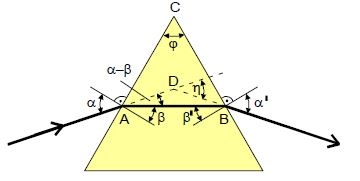
\includegraphics[width = 10cm]{img/symmetrisch.JPG}
		\caption{Symmetrischer Strahlengang durch ein Prisma \cite{anleitung}}
		\label{symmetrisch}
	\end{figure}

	Daraus lassen sich nun die folgenden Winkelbeziehungen ablesen.

	\begin{equation}
		\sphericalangle\mathrm{CAB} = 90 -\frac{\phi}{2} = 90 - \beta
	\end{equation}

	Weiterhin ergibt sich:

	\begin{equation}
		\alpha = \frac{\eta + \varphi}{2}
	\end{equation}

	Nun ergibt sich mit Snellius:

	\begin{equation}
		n = \frac{\sin(\frac{\eta+\varphi}{2})}{\sin(\frac{\varphi}{2})} \label{eqn:brechungsindex}
	\end{equation}

	Zur Bestimmmung der Winkel wird ein Goniometer verwendet (Abb. \ref{gonio}).

	\begin{figure}[!h]
		\centering
		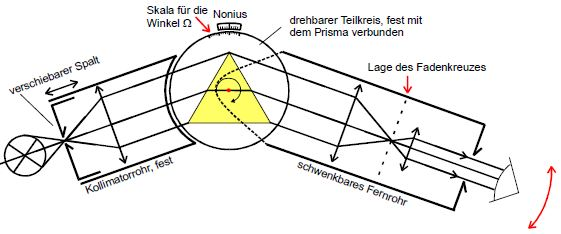
\includegraphics[width = 12cm]{img/gonio.JPG}
		\caption{Schematische Darstellung eines Prismen-Spektralapparates \cite{anleitung}}
		\label{gonio}
	\end{figure}

	Das Licht f"allt durch einen Spalt auf eine Sammellinse, wodurch parallele Strahlen erzeugt werden (Kollimator).
	Das Prisma bricht das Licht und der gebrochene Strahl gelangt in das Fernrohr. Die dortige Objektivlinse entwirft ein reelles Spaltbild in ihrer Brennebene und dieses kann mithilfe des Okulars beobachtet werden.
	In der Brennebene des Objektivs ist ein Fadenkreuz angebracht und dieses kann durch Schwenken des Fernrohres um die Goniometerachse mit dem Spaltbild zur Deckng gebracht werden kann.

	\subsection{Beschreibung des Messvorganges} % (fold)
	\label{sub:beschreibung_des_messvorganges}
	
	Nachdem ein scharfes Spaltbild im Fernrohr beobachtet wird, k"onnen die Gr"o"sen $\varphi$ und $\eta$ gemessen werden.

	\subsection{$\varphi$-Messung} % (fold)
	\label{sub:varphi_}
	
	\begin{figure}[!h]
		\centering
		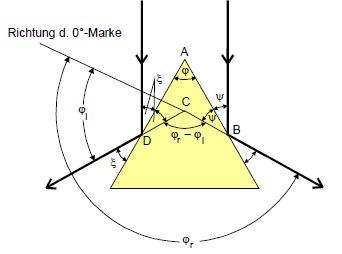
\includegraphics[width = 8cm]{img/phi.JPG}
		\caption{Skizze zur Bestimmung des Winkels $\varphi$ zwischen den brechenden Oberfl"achen. \cite{anleitung}}
		\label{fg:phi}
	\end{figure}

	Zur Messung des brechenden Winkels $\varphi$ wird das Prisma mit seiner brechenden Kante ungef"ahr auf das Kollimatorrohr ausgerichtet (Abb. \ref{fg:phi}).

	Das Fadenkreuz wird auf die Maxima der gebrochenen Strahlen gelegt und der dazugeh"orige Winkel $\varphi_\mathrm{l}$ notiert. Nun wird das Fernrohr auf die andere Seite gefahren und das Verfahren widerholt. Dort werden die Winkel $\varphi_\mathrm{r}$ notiert.

	F"ur den Winkel $\varphi$ ergibt sich:

	\begin{equation}
		\varphi = \frac{1}{2} ( \varphi_\mathrm{r} - \varphi_\mathrm{r} ) \label{eqn:phi}
	\end{equation}

	\subsubsection{$\eta$-Messung} % (fold)
	\label{sub:subsection_name}
	
	\begin{figure}[!h]
		\centering
		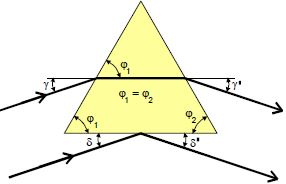
\includegraphics[width = 8cm]{img/eta.JPG}
		\caption{Verlauf des reflektierten und des gebrochenen Strahls bei einem symmetrischen Strahlengang an einem gleichschenkligen Prisma \cite{anleitung}.}
		\label{fg:eta}
	\end{figure}

	Nun kann der Winkel $\eta$ des Strahlenganges berechnet werden.
	F"ur diese Messung muss ein symmetrischer Strahlengang vorliegen (Abb. \ref{fg:eta}).
	Um diese Einstellung zu finden, muss die Stellung des Prismas solange um die Goniometerachse ver"andert werden, bis der reflektierte und der gebrochene Strahlengang zusammenfallen. Die Winkelstellung $\Omega_\mathrm{l}$ des Fernrohrs wird notiert.

	Die Richtung des ungebrochenen Strahls ist nicht mit hinreichender Genauigkeit bekannt, weshalb die Messung bei einer spiegelsymmetrischen Stellung des Prismas wiederholt wird. Der neue Winkel $\Omega_\mathrm{r}$ wird notiert.

	\begin{figure}[!h]
		\centering
		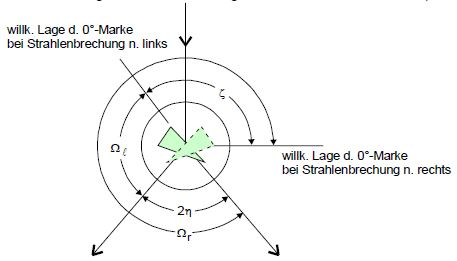
\includegraphics[width = 12cm]{img/omega.JPG}
		\caption{Darstellung der Messgr"o"sen $\Omega_\mathrm{l}$ und $\Omega_\mathrm{r}$ in Zusammenhang mit den beiden spiegelbildchen Prismenstellungen. \cite{anleitung}}
		\label{omega}
	\end{figure}

	Aus den Beziehungen in Abb. \ref{omega} ergibt sich f"ur den Winkel $\eta$:

	\begin{equation}
		\eta = 180 - (\Omega_\mathrm{r} - \Omega_\mathrm{l}) \label{eqn:eta}
	\end{equation}